% !TEX root =../thesis-letomes.tex

\chapter{Physical Modelling}
We need a chapter to formulate our hypotheses, and generally give a before-the-fact run-down of what the project and report will be like.

\section{CM-Centric Restricted 3-Body System (Earth-Moon)}

\subsection{Equations of Motion}

\subsection{Numerical Algorithm}


\section{Heliocentric Restricted 4-Body System (Sun-Earth-Mars)}
Simulating orbit from Earth to Mars requires a new model with at least four bodies: Sun, Earth, Mars and the Spacecraft. The coordinate system will be heliocentric and in spherical coordinates, and restricted meaning that the mass of the spacecraft is considered negligible compared to compared to the celestial masses, so we call this system the ``Heliocentric Restricted N-Body'' system. We will derive the equations of motion of the spacecraft by using Hamilton's equations, which naturally gives us a set of coupled first-order differential equations, and a set of conserved quantities as ``generalized momenta''.

\subsection{Spherical Coordinate System}
We adopt the spherical coordinate system which customary in astrodynamics. The conventions used is in \cref{fig:3D_Spherical}.

\begin{figure}[ht]
    \centering
    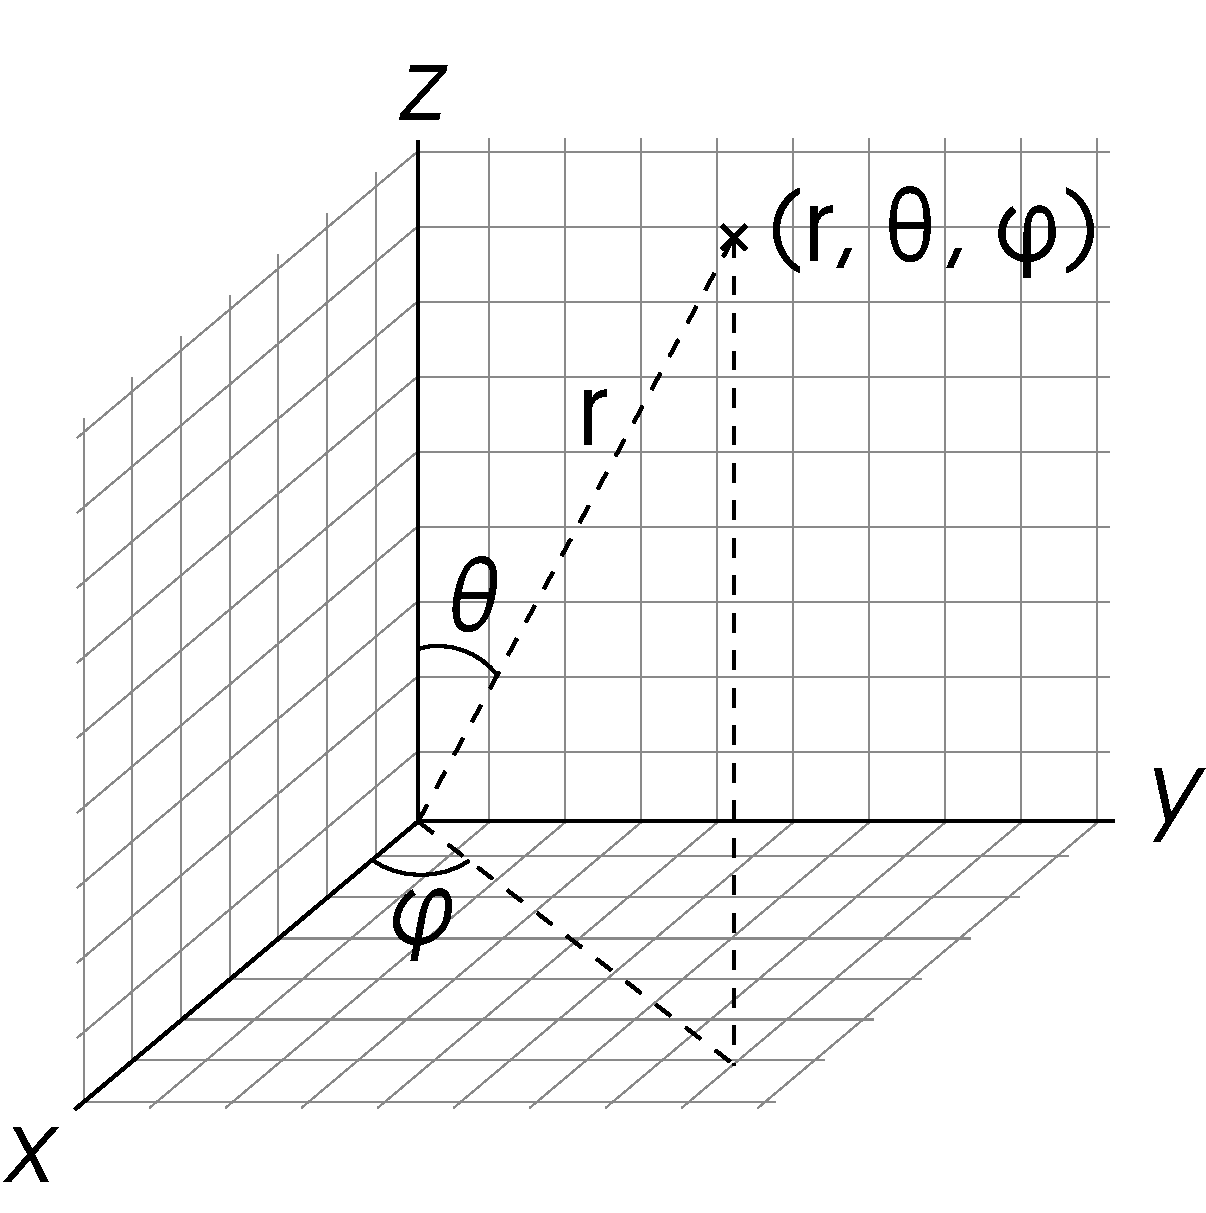
\includegraphics[width=0.50\linewidth]{fig/3D_Spherical}
    \caption{Spherical coordinates \((r, \theta, \phi)\). Radial distance \(r\), polar angle \(\theta\) (theta), and azimuthal angle \(\phi\) (phi). In our heliocentric system the sun is assumed to be stationary at the origin. Source: \cite{WikiSpherical}.}
    \label{fig:3D_Spherical}
\end{figure}

And the coordinate transform equations to and from the cartesian coordinate system are:

\begin{align}
    x &= r \sin{\theta}\cos{\phi}, \label{eq:x(q)} \\
    y &= r \sin{\theta}\sin{\phi}, \label{eq:y(q)}\\
    z &= r \cos{\theta}, \label{eq:z(q)}
\end{align}

and

\begin{align}
    r &= \sqrt{x^2 + y^2 + z^2}, \label{eq:r(x,y,z)}\\
    \theta &= \arccos{\frac{z}{r}}, \label{eq:theta(x,y,z)}\\
    % \arctan{\frac{y}{x}}, \qquad \theta  \in [0, 2\pi]
    \phi &= 
    \begin{cases}
    \arctan{\frac{y}{x}} & \text{if \(x \geq 0\) \qquad \qquad \ \ \ (Q1, Q4),}
    \\
    \arctan{\frac{y}{x}}+\pi & \text{if \(x \leq 0,\ y \geq 0\) \qquad (Q2),}
    \\
    \arctan{\frac{y}{x}}-\pi & \text{if \(x \leq 0,\ y \leq 0\) \qquad (Q3).}
    \end{cases} \label{eq:phi(x,y,z)}
\end{align}

where \(r \in [0, \infty]\), \(\theta \in [0, \pi]\) and \(\phi \in [0, 2\pi]\).

For the calculation of kinetic in the next section we will need the position vector, unit vectors in spherical coordinates, and the Jacobians.

The position vector in spherical coordinates is
\begin{align}
    \vec{r}(r, \theta, \phi) &= x \xhat + y \yhat + z \zhat \\
    \Leftrightarrow \vec{r}(r, \theta, \phi) &= r \sin{\theta}\cos{\phi} \xhat + r \sin{\theta}\sin{\phi} \yhat + r \cos{\theta} \zhat. \label{eq:position-vec-spherical}
\end{align}

The various coordinate derivatives of the position vector is
\begin{align}
    \pd{\vec{r}}{r} &= \sin{\theta}\cos{\phi} \xhat + \sin{\theta}\sin{\phi} \yhat + \cos{\theta} \zhat \quad &\text{and} \quad &\left| \pd{\vec{r}}{r} \right| = 1 \label{eq:position-derived-r} \\
    \pd{\vec{r}}{\theta} &= r \cos{\theta}\cos{\phi} \xhat + r \cos{\theta}\sin{\phi} \yhat - r \sin{\theta} \zhat \quad &\text{and} \quad &\left| \pd{\vec{r}}{\theta} \right| = r \label{eq:position-derived-theta} \\
    \pd{\vec{r}}{\phi} &= -r\sin{\theta}\sin{\phi} \xhat + r\sin{\theta}\cos{\phi} \zhat \quad &\text{and} \quad &\left| \pd{\vec{r}}{\phi} \right| = r\sin{\theta} \label{eq:position-derived-phi}
\end{align}

So the unit vectors in spherical coordinates are
\begin{align}
    \rhat = \dfrac{\pd{\vec{r}}{r}}{\left| \pd{\vec{r}}{r} \right| } &= \sin{\theta}\cos{\phi} \xhat + \sin{\theta}\sin{\phi} \yhat + \cos{\theta} \zhat \label{eq:r-hat}\\
    \thetahat = \dfrac{\pd{\vec{r}}{\theta}}{\left| \pd{\vec{r}}{\theta} \right| } &= \cos{\theta}\cos{\phi} \xhat + \cos{\theta}\sin{\phi} \yhat - \sin{\theta} \zhat \label{eq:theta-hat}\\
    \phihat = \dfrac{\pd{\vec{r}}{\phi}}{\left| \pd{\vec{r}}{\phi} \right| } &= -\sin{\phi} \xhat + \cos{\phi} \zhat \label{eq:phi-hat}
\end{align}

\subsection{HR4B Equations of Motion}
We will follow the 5-step process of arriving at Hamilton's equations outlined in \cref{apx:hamiltons}.

\subsubsection{Step 1: Lagrangian \(L\)}
The kinetic energy of the system is
\begin{align}
    T = \frac{1}{2} m_s v^2.
\end{align}

In general the total derivative of a vector is:

\begin{align}
    \vec{v} &= \od{\vec{r}}{t} = \sum\limits_{i} \pd{\vec{r}}{q_i} \od{q_i}{t}, \\
      &= \sum\limits_{i} \left|\pd{\vec{r}}{q_i}\right| \frac{\pd{\vec{r}}{q_i}}{\left|\pd{\vec{r}}{q_i}\right|} \od{q_i}{t}, \\
      &= \sum\limits_{i} \left|\pd{\vec{r}}{q_i}\right| \od{q_i}{t} \unitvector{q}_i, \\
      &= \sum\limits_{i} \left|\pd{\vec{r}}{q_i}\right| \dot{q_i} \unitvector{q}_i,
    \end{align}

where we have used that a unit vector for any coordinate system is \(\frac{\pd{\vec{r}}{q_i}}{\left|\pd{\vec{r}}{q_i}\right|} = \unitvector{q}_i\).
We can now use the derivatives of the position vector we found earlier in \cref{eq:position-derived-r,eq:position-derived-theta,eq:position-derived-phi}, to substitute for \(\left|\pd{\vec{r}}{q_i}\right|\). We don't have to substitute in \(\unitvector{q}_i\) since our unit vectors are orthogonal, so they will yield either 0 or 1 when we square \(v\). So for the spherical coordinates we get:

\begin{align}
    \vec{v} = \dot{r}\rhat + r\dot{\theta}\thetahat + r\sin{\theta}\,\dot{\phi}\phihat
\end{align}

so

\begin{align}
    v^2 = \dot{r}^2 + r^2\dot{\theta}^2 + r^2\sin^2{\theta}\,\dot{\phi}^2
\end{align}

so we get

\begin{align}
    T = \frac{1}{2} m_s (\dot{r}^2 + r^2\dot{\theta}^2 + r^2\sin^2{\theta}\,\dot{\phi}^2).
\end{align}

The gravitational potential is \todoref{find some non-wikipedia reference here}

\begin{align}
    V = -G m_s \sum\limits_{i} \frac{M_i}{\left| \vec{r} - \vec{r_i} \right|},
\end{align}
where \(i\) denotes the celestial bodies acting on the spacecraft, i.e. in our system Sun, Earth and Mars.

So we finally get the Lagrangian

\begin{align}
    L &= T - V \\
    \Leftrightarrow L &= \frac{1}{2} m_s (\dot{r}^2 + r^2\dot{\theta}^2 + r^2\sin^2{\theta}\,\dot{\phi}^2) + G m_s \sum\limits_{i} \frac{M_i}{\left| \vec{r} - \vec{r_i} \right|}
\end{align}

\subsubsection{Step 2: Generalized Momenta \(p_i\)}
\begin{align}
    p_r &= \pd{L}{\dot{r}} = m_s \dot{r} \label{eq:pr} \\
    p_\theta &= \pd{L}{\dot{\theta}} = m_s r^2 \dot{\theta} \label{eq:ptheta} \\
    p_\phi &= \pd{L}{\dot{\phi}} = m_s r^2 \sin^2{\theta} \dot{\phi} \label{eq:pphi}
\end{align}

\subsubsection{Step 3: \(\dot{q} = \dot{q}_i(\vec{q}, \vec{p}, t)\)}
\begin{align}
    \dot{r} &= \frac{p_r}{m_s} \\
    \dot{\theta} &= \frac{p_\theta}{m_s r^2} \\
    \dot{\phi} &= \frac{p_\phi}{m_s r^2 \sin^2{\theta}}
\end{align}

We can now rewrite \(L\) to make it independent of \(\dot{q}\) by substituting the expressions above:

\begin{align}
    T &= \frac{1}{2} m_s (\dot{r}^2 + r^2\dot{\theta}^2 + r^2\sin^2{\theta}\,\dot{\phi}^2) \\
    &= \frac{1}{2} m_s \left(\frac{p_r^2}{m_s^2} + r^2\frac{p_\theta^2}{m_s^2 r^4} + r^2\sin^2{\theta}\frac{p_\phi^2}{m_s^2 r^4 \sin^4{\theta}} \right) \\
    &= \frac{p_r^2}{2 m_s} + \frac{p_\theta^2}{2 m_s r^2} + \frac{p_\phi^2}{2 m_s r^2 \sin^2{\theta}} \\
\end{align}

So we have

\begin{align}
    L = \frac{p_r^2}{2 m_s} + \frac{p_\theta^2}{2 m_s r^2} + \frac{p_\phi^2}{2 m_s r^2 \sin^2{\theta}} + G m_s \sum\limits_{i} \frac{M_i}{\left| \vec{r} - \vec{r_i} \right|}
\end{align}

\subsubsection{Step 4: Hamiltonian \(H\)}
\begin{align}
    H(\vec{q}, \vec{p}, t) &= \sum\limits_{i}p_i \dot{q_i} - L \\
    &= \sum\limits_{i}p_i \dot{q_i}(\vec{q}, \vec{p}, t) - L \\
    &= p_r \frac{p_r}{m_s} + p_\theta \frac{p_\theta}{m_s r^2} + p_\phi + \frac{p_\phi}{m_s r^2 \sin^2{\theta}} \nonumber \\
    &- \left( \frac{p_r^2}{2 m_s} + \frac{p_\theta^2}{2 m_s r^2} + \frac{p_\phi^2}{2 m_s r^2 \sin^2{\theta}} + G m_s \sum\limits_{i} \frac{M_i}{\left| \vec{r} - \vec{r_i} \right|} \right) \\
    \Leftrightarrow H &= \frac{p_r^2}{2 m_s} + \frac{p_\theta^2}{2 m_s r^2} + \frac{p_\phi^2}{2 m_s r^2 \sin^2{\theta}} - G m_s \sum\limits_{i} \frac{M_i}{\left| \vec{r} - \vec{r_i} \right|}
\end{align}

At this point we want to expand the expression \(\left| \vec{r} - \vec{r_i} \right|\) in anticipation of needing to differentiate \(H\) with respect to the coordinates. Using the equations for the \(x, y, z\) coordinates \cref{eq:x(q),eq:y(q),eq:z(q)} we get

\begin{align}
    d_i = \left|\vec{r} - \vec{r}_i \right| &= \sqrt{(x-x_i)^2 + (y-y_i)^2 + (z-z_i)^2}
\end{align}
and
\begin{align}
    (x-x_i)^2 &= (r\sin{\theta}\cos{\phi} - r\sin{\theta}\cos{\phi})^2 \nonumber \\
    &= \tikz[baseline]{
        \node[fill=orange!20,anchor=base]
        {\(r^2\sin^2{\theta}\cos^2{\phi}\)}
    } + \tikz[baseline]{
        \node[fill=red!20,anchor=base]
        {\(r_i^2\sin^2{\theta_i}\cos^2{\phi_i}\)}
    } - 2r r_i \sin{\theta}\sin{\theta_i}\cos{\phi}\cos{\phi_i} \label{eq:x-dist-squared} \\
    (y-y_i)^2 &= (r\sin{\theta}\sin{\phi} - r\sin{\theta}\sin{\phi})^2 \nonumber \\
    &= \tikz[baseline]{
        \node[fill=orange!20,anchor=base]
        {\(r^2\sin^2{\theta}\sin^2{\phi}\)}
    } + \tikz[baseline]{
        \node[fill=red!20,anchor=base]
        {\(r_i^2\sin^2{\theta_i}\sin^2{\phi_i}\)}
    } - 2r r_i \sin{\theta}\sin{\theta_i}\sin{\phi}\sin{\phi_i} \label{eq:y-dist-squared} \\
    (z-z_i)^2 &= (r\cos{\theta} - r\cos{\theta})^2 \nonumber \\
    &= \tikz[baseline]{
        \node[fill=orange!20,anchor=base]
        {\(r^2\cos^2{\theta}\)}
    } + \tikz[baseline]{
        \node[fill=red!20,anchor=base]
        {\(r_i^2\cos^2{\theta_i}\)}
    } - 2r r_i \cos{\theta}\cos{\theta_i}. \label{eq:z-dist-squared}
\end{align}
Now adding all three \cref{eq:x-dist-squared,eq:y-dist-squared,eq:z-dist-squared} the orange terms add to \(r^2\) and the red terms add to \(r_i^2\) and we get

\begin{align}
    d_i &= \sqrt{
        \tikz[baseline]{\node[fill=orange!20,anchor=base]{\(r^2\)}}
        + \tikz[baseline]{\node[fill=red!20,anchor=base]{\(r_i^2\)}}
        -2r r_i(\cos{\theta}\cos{\theta_i}+\sin{\theta}\sin{\theta_i}(
            \tikz[baseline]{\node[fill=blue!20,anchor=base]{
                \(\cos{\phi}\cos{\phi_i} + \sin{\phi}\sin{\phi_i}\)}}
        ))
    } \\
    &= \sqrt{(r - r_i)^2(\cos{\theta}\cos{\theta_i}+\sin{\theta}\sin{\theta_i}(\cos{\phi - \phi_i}))},
\end{align}
where the blue factor was simplified using the sum rule \\
\(\cos{\alpha}\cos{\beta} + \sin{\alpha}\sin{\beta} = cos{\alpha-\beta}\)\cite{WeissteinTrig}.

So we can finally express \(H\) as
\begin{equation}
    \begin{aligned}
        H &= \frac{p_r^2}{2 m_s} + \frac{p_\theta^2}{2 m_s r^2} + \frac{p_\phi^2}{2 m_s r^2 \sin^2{\theta}} \\
        &- G m_s \sum\limits_{i} \frac{M_i}{\sqrt{(r - r_i)^2\left[\cos{\theta}\cos{\theta_i}+\sin{\theta}\sin{\theta_i}\cos{(\phi - \phi_i})\right]}}
    \end{aligned}
\end{equation}

\subsubsection{Step 5: Hamilton's Equations}
\begin{align}
    \dot{r} = \pd{H}{p_r} &= \frac{p_r}{m_s} \label{eq:rdot} \\[0.3cm]
    \dot{\theta} = \pd{H}{p_\theta} &= \frac{p_\theta}{m_s r^2} \label{eq:thetadot} \\[0.3cm]
    \dot{\phi} = \pd{H}{p_\phi} &= \frac{p_\phi}{m_s r^2 \sin^2{\theta}} \label{eq:phidot}  \\[0.3cm]
    \begin{split}
        \dot{p}_r = -\pd{H}{q_r} &= \frac{p_\theta^2}{m_s r^3} + \frac{p_\phi^2}{m_s r^3 \sin^2{\theta} } \\
        &+ G m_s \sum\limits_{i} M_i \frac{-\left[r - r_i \left(\cos{\theta}\cos{\theta_i} + \sin{\theta}\sin{\theta_i}\cos{(\phi - \phi_i)}\right) \right]}{\left[(r - r_i)^2 \left(\cos{\theta}\cos{\theta_i} + \sin{\theta}\sin{\theta_i}\cos{(\phi - \phi_i)} \right) \right]^{3/2}} \label{eq:prdot}
    \end{split} \\[0.3cm]
    \begin{split}
        \dot{p}_\theta = -\pd{H}{q_\theta} &= \frac{p_\phi^2}{m_s r^2 \sin^2{\theta} \tan{\theta}} \\
        &+ G m_s \sum\limits_{i} M_i \frac{- r r_i \left[\sin{\theta}\cos{\theta_i} + \cos{\theta}\sin{\theta_i}\cos{(\phi - \phi_i)} \right]}{\left[(r - r_i)^2 \left(\cos{\theta}\cos{\theta_i} + \sin{\theta}\sin{\theta_i}\cos{(\phi - \phi_i)} \right) \right]^{3/2}} \label{eq:pthetadot}
    \end{split} \\[0.3cm]
    \begin{split}
        \dot{p}_r = -\pd{H}{q_r} &= \frac{p_\theta^2}{m_s r^3} + \frac{p_\phi^2}{m_s r^3 \sin^2{\theta} } \\
        &+ G m_s \sum\limits_{i} M_i \frac{-r r_i \sin{\theta}\sin{\theta_i}\sin{(\phi - \phi_i)}}{\left[(r - r_i)^2 \left(\cos{\theta}\cos{\theta_i} + \sin{\theta}\sin{\theta_i}\cos{(\phi - \phi_i)} \right) \right]^{3/2}} \label{eq:pphidot}
    \end{split}
\end{align}

Those are our equations of motion. However before we try to solve them, we will remove all units.

\subsection{HR4B Equations of Motion - Nondimensionalized}
We will now choose suitable characteristic units, which has a number of benefits:
\begin{itemize}
    \item The equations gets slightly simplified
    \item The order of the effects of different forces in the system becomes more apparent.
    \item Many of the calculations in numerical algorithms happens at an order of about 1. 
\end{itemize}

The characteristic units are chosen as:
\begin{align}
    \text{Unit length: } k_r &= a_{\Earth}\ {\color{gray} \approx \SI{1.50e8}{\km}}  \\[0.2cm]
    \text{Unit time: } k_t &= T_{\Earth} = \frac{2\pi}{\omega_\Earth} = 2\pi \sqrt{\frac{a_\Earth^3}{G M_\Sun}}\ {\color{gray} \approx \SI{3.16e7}{\s} \text{ (1 year)}} \\[0.2cm]
    \text{Unit speed: } k_v &= \frac{k_r}{k_t} = \frac{a_\Earth \omega_\Earth}{2\pi} = \frac{1}{2\pi} \sqrt{\frac{G M_\Sun}{a_\Earth}}\ {\color{gray} \approx \SI{4.74}{\km/\s}}
\end{align}
where \(a_\Earth\) is the semi-major axis of Earth's orbit in kilometers, see \cref{fig:earth-semi-major-axis}, \(T_\Earth\) is Earth's orbital period (i.e. 1 year) in seconds and the characteristic speed thus becomes Earth's average orbital speed with respect to the sun.

We don't need a characteristic mass \(m_s\) since the mass cancels out in the equations of motion for the quantity we care about, delta-v.

The unit for time is expressed in seconds because we found heuristically we needed time steps on the order of \(\SI{1}{\s}\) to maintain an error per step of about \num{10e-9}.

The unit for length is expressed in kilometers because it is customary to use \si{\km/\s} as unit of speed for celestial objects.

\begin{figure}[ht]
    \centering
    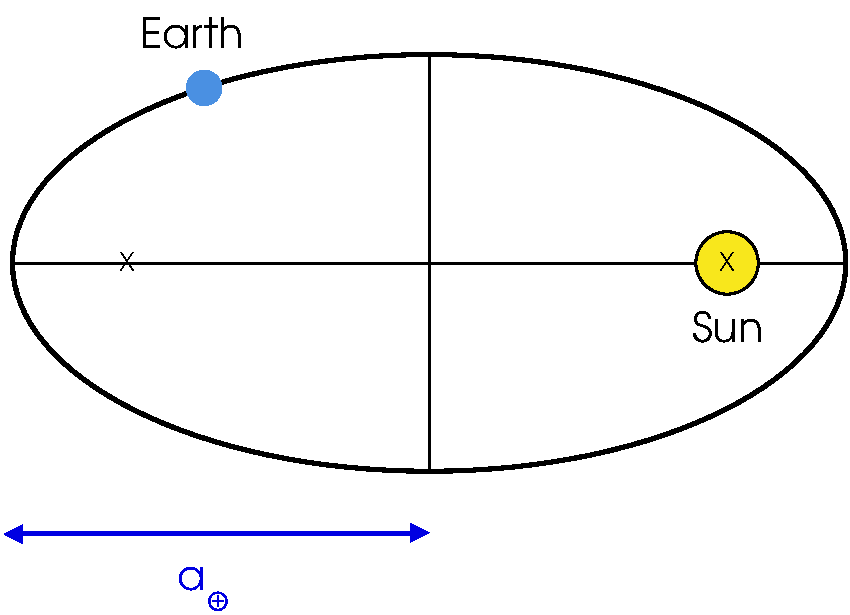
\includegraphics[width=0.60\linewidth]{fig/earth-semi-major-axis}
    \caption{Semi-major axis of Earth's elliptical orbit, used as the characteristic length of the system}
    \label{fig:earth-semi-major-axis}
\end{figure}

Looking at the \(p_i\) from \cref{eq:pr,eq:ptheta,eq:pphi} we can infer their units:

\begin{align}
    k_{pr} &= \frac{k_m}{k_r k_t} \\[0.2cm]
    k_{p\theta} &= \frac{k_m k_r^2}{k_t} = k_{pr} k_r \\[0.2cm]
    k_{p\phi} &= k_{p\theta}
\end{align}

We now introduce the quantity

\begin{equation}
    b_i = \frac{p_i}{m_s}.
\end{equation}
It proves useful to introduce into Hamilton's equations because the mass cancels out (as expected from Newton's 2nd Law, and thus removes the need for introducing  selecting characteristic mass \(k_m\). We will treat the interpretation later. \(b_i\) has units:

\begin{align}
    k_{br} = \frac{k_{pr}}{k_m} = \frac{k_r}{k_t} \\[0.2cm]
    k_{b\theta} = \frac{k_{p\theta}}{k_m} = \frac{k_r^2}{k_t} \\[0.2cm]
    k_{b\phi} = \frac{k_{p\phi}}{k_m} = \frac{k_r^2}{k_t}
\end{align}

To be continued... (see r4b-spherical.pdf)

% For \cref{eq:rdot,eq:thetadot,eq:phidot} we set \(b_i = \frac{p_i}{m_s}\) and nondimensionalize:

% \begin{align}
%     \od{r}{t} = \frac{p_r}{m_s} \\
%     \Leftrightarrow \od{r}{t} = b_r \\
%     \Leftrightarrow \od{r}{t} = b_r \\ 
% \end{align}



\subsection{Numerical Algorithm}
